\documentclass{article}

\usepackage{fancyhdr}

\RequirePackage{epsfig}

\RequirePackage{graphics}

\ExecuteOptions{dvipsone}

\pagestyle{fancy}
\lhead{}
\chead{Developing A Command Language Using XMF}
\rhead{\thepage}
\cfoot{(c) 2004 Ceteva Ltd.}

\title{Developing A Command Language Using XMF}

\author{Ceteva Ltd.}

\begin{document}

\maketitle

\tableofcontents

\section{The Language Design Space}

{\em Language} is something that we use to convey meaning. A language
consists of a collection of syntax rules that determine the form of
communication in the language and a collection of semantic rules that
associate communications with meaning. In order that a language definition
is well-formed, it must have both syntax and semantics.

Syntax rules can take a number of forms depending on the intended phrase 
structure of the language. Syntax may be {\em concrete} (human-centric)
or {\em abstract} (machine-centric). Standard technologies have been
developed for expressing textual concrete syntax (the BNF family) and
to a lesser extent for expressing graphical concrete syntax (such as
graph grammars).

Semantic rules offer a greater variety of options depending on the nature
of the language. In broad terms, languages are either {\em operational}
or {\em non-operational}. An operational language is one that controls
the execution of some form of machine and as a result has semantics
that relate phrases in the language to machine executions. A non-operational 
language is not restricted in terms of its semantics. This note is concerned 
with operational languages. 

The semantics of an operational language is defined by relating the syntax domain
of the language to a semantic domain. A number of different styles can be used
for the operational definition. Two extreme examples are:

\begin{enumerate}

\item The semantic domain is defined as a set of values produced by 
performing the syntax phrases. The semantic relationship takes the form of
an interpreter written in some other language. This is a very attractive
way of defining the operational semantics of a language since the
semantics can be implemented directly. A drawback of this approach is that 
the interpreter tends to be relatively complex and the semantics of the
auxiliary language must be included in the language definition.

\item The semantic domain is defined as a set of machine calculations
produced by executing the syntax phrases on the intended target machine.
This is to be contrasted with writing an interpreter that maps the
syntax domain to the semantic domain. The interpreter approach leads to 
a complex semantic relationship and a simple semantic domain whereas the
complexity is reversed using the calculational approach.

\end{enumerate}
This note is concerned with writing interpreters (translators and compilers).

When defining an interpretive semantics for a language we often have a
similar language at hand (at least the language we are writing the interpreter 
in). We then have the choice as to whether the syntax structures are
directly interpreted or whether they are translated to syntax phrases in the
existing language. The advantage of a translational approach is that the
execution engine for the target language already exists and is probably
more efficient than any interpreter we could write for the source language.
Compilers are translators for languages where the target language is usually
highly optimized and very different from the source language. In principle,
however, there is no essential difference between a transator and a compiler.
A language that uses the translational approach to target a sub-language
of itself is often referred to as {\em desugaring} the source language.

This note describes how XMF technologies can be used to support a translational
approach to language development. A simple command language is used as the
case study.

\section{XCom - A Simple Command Language}

\label{Intro}

{\em XCom} is a simple command language with values that are either
records or are atomic. An atomic data value is a string, integer or boolean.
A record is a collection of named values. XCom is block-structured where
blocks contain type definitions and value definitions. XCom has simple 
control structures: conditional statements and loops. The following is a
simple example XCom program that builds a list of even numbers from 2 to 100:
\begin{verbatim}
begin
  type Pair is head tail end
  type Nil is end
  value length is 100 end
  value list is new Nil end
  while length > 0 do
    begin
      if length % 2 = 0
      then
        begin
          value pair is new Pair end
          pair.head := length;
          pair.tail := list;
          list := pair;
        end
      end;
      length := length - 1;
    end
end
\end{verbatim}
The definition of XCom is structured as a collection of XMF packages. The {\tt Values}
package defines the semantic domain for XCom; it contains classes for each type of
program value. Executable program phrases in XCom are divided into two categories: 
{\tt Expressions} and {\tt Statements}. Expressions evaluate to produce XCom values.
Statements are used to control the flow of execution and to update values.
\begin{verbatim}
@Package XCom
  @Package Values end
  @Package Expressions end
  @Package Statements end
end
\end{verbatim}
The rest of this section defines the syntax of XCom by giving the basic class definitions
and the XBNF grammar rules for the language constructs.

\subsection{XCom Values}

XCom expressions evaluate to produce XCom values. Values are defined in the {\tt Values} package
and which is the {\em semantic domain} for XCom. Values are either atomic: integers and booleans, or
are records. We use a simple representation for records: a sequence of values indexed by names.

XCom records are created by instantiating XCom record types. A record type is a sequence of names.
Types raise an interesting design issue: should the types be included as part of the semantic domain
since evaluation of certain XCom program phrases give rise to types that are used later in the
execution to produce records. The answer to the question involves the phase distinction that
occurs between {\em static} analysis (or execution) and {\em dynamic} execution. Types are often
viewed as occurring only during static analysis; although this is not always the case.
We will show how the semantics of XCom can be defined with and without dynamic types.

All values are instances of sub-classes of the class {\tt Value}:
\begin{verbatim}
context Values
 @Class Value
   @Attribute value : Element end
   @Constructor(value) ! end
 end
\end{verbatim}
Atomic values are either booleans or integers. Each class defines operations
that the semantic domain provides for manipulating XCom values. The classes below show
the structure and a representative sample of operations:
\begin{verbatim}
context Values
  @Class Bool extends Value
    @Operation binAnd(Bool(b))
      Bool(value and b)
    end
    @Operation binOr(Bool(b))
      Bool(value or b)
    end
  end
\end{verbatim}

\begin{verbatim}
context Values
  @Class Int extends Value
    @Operation binAdd(Int(n))
      Int(value + n)
    end
  end
\end{verbatim}
Record types are sequences of names. A type provides a {\tt new} operation that instantiates the
type to produce a new record. This operation is only meaningful if we have dynamic types:
\begin{verbatim}
context Values
  @Class Type extends Value
    @Attribute names : Seq(String) end
    @Constructor(names) ! end
    @Operation new()
      Record(self,names->collect(n | Seq{n | null}))
    end
  end
\end{verbatim}
Records are sequences of values indexed by names; the names are found by navigating to the
type of the record:
\begin{verbatim}
context Values
  @Class Record extends Value
    @Attribute type : Type end
    @Attribute fields : Seq(Element) end
    @Constructor(type,fields) ! end
    @Operation lookup(name:String)
      fields->at(type.names->indexOf(name))
    end
    @Operation update(name:String,value:Element)
      fields->setAt(type.names->indexOf(name),value)
    end
  end
\end{verbatim}

\subsection{XCom Expressions}

XCom expressions are program phrases that evaluate to produce XCom values. The following classes
define the expression types:
\begin{verbatim}
context Expressions
  @Class Exp
  end
end
\end{verbatim}
A binary expression has a left and right sub-expression and an operation. The name of the operation
is represented as a string:
\begin{verbatim}
context Expressions
  @Class BinExp extends Exp
    @Attribute op : String end
    @Attribute left : Exp end
    @Attribute right : Exp end
    @Constructor(op,left,right) ! end
  end
\end{verbatim}
An atomic constant expression is either an integer or a boolean:
\begin{verbatim}
context Expressions
  @Class Const extends Exp
    @Attribute value : Element end
    @Constructor(value) ! end
  end
end
\end{verbatim}
A new record is produced by performing a {\tt new} expression. The type to instantiate is
given as a string. An alternative representation for types in {\tt new} expressions would
be to permit an arbitrary expression that {\em evaluates} to produce a type. This design choice
would rule out static typing and force the language to have dynamic types. We wish to use
XCom to illustrate the difference between dynamic and static types in semantic definitions
so we use strings to name types in {\tt new} expressions:
\begin{verbatim}
context Expressions
  @Class New extends Exp
    @Attribute type : String end
    @Constructor(type) ! end
  end
end
\end{verbatim}
A variable is just a name:
\begin{verbatim}
context Expressions
  @Class Var extends Exp
    @Attribute name : String end
    @Constructor(name) ! end
  end
\end{verbatim}
A record field ref is:
\begin{verbatim}
context Expressions
  @Class FieldRef extends Exp
    @Attribute value : Exp end
    @Attribute name : String end
    @Constructor(value,name) ! end
  end
\end{verbatim}
The concrete syntax of expressions is defined by the XBNF grammar for the class {\tt Exp}.
The grammar parses the expression syntax and synthesizes instances of the expression classes:
\begin{verbatim}
context Exp
 @Grammar    
   // Start at Exp. Logical operators bind weakest.
   Exp ::= e = ArithExp [ op = LogicalOp l = Exp { BinExp(op,e,l) } ].
   LogicalOp ::= 'and' { "and" } | 'or' { "or" }.
   // The '.' for field ref binds tighter than '+' etc.
   ArithExp ::= e = FieldRef [ op = ArithOp a = FieldRef { BinExp(op,e,a) } ].
   ArithOp ::= '+' { "+" }.
   // A field reference '.' optionally follows an atomic expression.
   FieldRef ::= e = Atom ('.' n = Name { FieldRef(e,n) } | { e }).
   // Atomic expressions can be arbitrary exps if in ( and ).
   Atom ::= Const | Var | New | '(' Exp ')'.
   Const ::= IntConst | BoolConst.
   IntConst ::= i = Int { Const(i) }.
   BoolConst ::= 'true' { Const(true) } | 'false' { Const(false) }.
   Var ::= n = Name { Var(n) }.
   New ::= 'new' n = Name { New(n) }.
 end
\end{verbatim}

\subsection{XCom Statements}

XCom statements are used to:
\begin{itemize}
\item Introduce new names associated with either types or values.
\item Control the flow of execution.
\item Perform side effects on records.
\end{itemize}
The following classes define the statement types for XCom:
\begin{verbatim}
context Statements
  @Class Statement
  end
end
\end{verbatim}
A block (as in Pascal or C) contains local definitions. Names introduced in a block
are available for the rest of the statements in the block (including sub-blocks) but are
not available when control exits from the block:
\begin{verbatim}
context Statements
  @Class Block extends Statement
    @Attribute statements : Seq(Statement) end
    @Constructor(statements) ! end
  end
end
\end{verbatim}
A declaration introduces either a type or a value binding:
\begin{verbatim}
context Statements
  @Class Declaration isabstract extends Statement
    @Attribute name : String end
  end
end
\end{verbatim}
A type declaration associates a type name with a sequence of field names. To keep things
simple we don't associate fields with types:
\begin{verbatim}
context Statements
  @Class TypeDeclaration extends Declaration
    @Attribute names : Seq(String) end
    @Constructor(name,names) ! end
  end
end
\end{verbatim}
A value declaration associates a name with a new value. The value is produced by performing
an expression at run-time:
\begin{verbatim}
context Statements
  @Class ValueDeclaration extends Declaration
    @Attribute value : Exp end
    @Constructor(name,value) ! end
  end
end
\end{verbatim}
A while statement involves a test and a body:
\begin{verbatim}
context Statements
  @Class While extends Declaration
    @Attribute test : Exp end
    @Attribute body : Statement end
    @Constructor(test,body) ! end
  end
end
\end{verbatim}
An if statement involves a test, a then-part and an else-part:
\begin{verbatim}
context Statements
  @Class If extends Declaration
    @Attribute test : Exp end
    @Attribute thenPart : Statement end
    @Attribute elsePart : Statement end
    @Constructor(test,elsePart) ! end
  end
end
\end{verbatim}

\begin{verbatim}
context Statements
  @Class FieldUpdate extends Declaration
    @Attribute record : Exp end
    @Attribute name : Exp end
    @Attribute value : Exp end
    @Constructor(record,name,value) ! end
  end
end
\end{verbatim}

\begin{verbatim}
context Statements
  @Class Update extends Declaration
    @Attribute name : String end
    @Attribute value : Exp end
    @Constructor(name,value) ! end
  end
end
\end{verbatim}

\begin{verbatim}
context Statement
  @Grammar extends Exp.grammar
    Statement ::= Block | Declaration | While | If | Update | FieldUpdate.
    Block ::= 'begin' s = Statement* 'end' { Block(s) }.
    Declaration ::= TypeDeclaration | ValueDeclaration.
    TypeDeclaration ::= 'type' n = Name 'is' ns = Name* 'end' { 
      TypeDeclaration(n,ns) }.
    ValueDeclaration ::= 'value' n = Name 'is' e = Exp 'end' { 
      ValueDeclaration(n,e) }.
    FieldUpdate ::= e = Exp '.' n = Name ':=' v = Exp ';' {
      FieldUpdate(e,n,v) }.
    While ::= 'while' e = Exp 'do' s = Statement 'end' {
      While(e,s) }.
    If ::= 'if' e = Exp 'then' s1 = Statement 'else' s2 = Statement 'end' {
      If(e,s1,s2) }.
    Update ::= n = Name ':=' e = Exp ';' {
      Update(n,e) }.
  end
\end{verbatim}

\section{An Evaluator for XCom}

As described in the introducion we are interested in defining XCom operational
semantics. We will do this in a number of different ways in the rest of this note.
The first, and possibly most straightforward, approach is to define an {\em interpreter} for
XCom in the XOCL language. This involves writing an {\tt eval} operation for each of the
XCom syntax classes. The {\tt eval} operation must be parameterized with respect to
any context information that is required to perform the evaluation. An XCom program {\tt p}
is then evaluated in a context {\tt e} by: {\tt p.eval(e)}.

\subsection{Evaluating Expressions}
Expression evaluation is defined by adding {\tt eval} operations to each class
in {\tt Expressions} as follows:
\begin{verbatim}
context Exp 
  @AbstractOp eval(env:Env):Value
  end
\end{verbatim}
Evaluation of a constant produces the appropriate semantic domain value:
\begin{verbatim}
context Const
  @Operation eval(env)
    @TypeCase(value)
      Boolean do Bool(value) end
      Integer do Int(value) end
    end
  end
\end{verbatim}
Evaluation of a variable involves looking up the current value. The value is found in the
current context of evaluation: this must contain associations between variable names and 
their values. This is the only thing required of the XCom evaluation context and therefore
we represent the context as an {\em environment} of variable bindings:
\begin{verbatim}
context Var
  @Operation eval(env)
    env.lookup(name)
  end
\end{verbatim}
Evaluation of a binary expression involves evaluation of the sub-expressions and then
selecting an operation based on the operation name. The following shows how XCom semantics
is completely based on XOCl semantics since {\tt +} in XCom is performed by {\tt +} in XOCL.
\begin{verbatim}
context BinExp
  @Operation eval(env)
    @Case op of
      "and" do left.eval(env).binAnd(right.eval(env)) end
      "or"  do left.eval(env).binOr(right.eval(env)) end
      "+"   do left.eval(env).binAdd(right.eval(env)) end
    end
  end
\end{verbatim}
Creation of new records is performed by evaluaing a {\tt new} expression. The interpreter has
dynamic types so the type to instantiate is found by looking up the type name in the current 
environment:
\begin{verbatim}
context New
  @Operation eval(env)
    env.lookup(type).new()
  end
\end{verbatim}
Field reference is defined as follows:
\begin{verbatim}
context FieldRef
  @Operation eval(env)
    value.eval(env).lookup(name)
  end
\end{verbatim}

\subsection{Evaluating Statements}

XCom statements are performed in order to introduce new names, control flow or to update a record field.
Statements are defined to evaluate in a context and must observe the rules of scope that require 
variables are local to the block that introduces them. The context of execution is an environment;
evaluation of a statement may update the supplied environment, so statement evaluation returns
an environment:
\begin{verbatim}
context Statement
  @AbstractOp eval(env):Env
  end
\end{verbatim}
A value declaration evaluates the expression part and then extends the supplied environment with a new
binding:
\begin{verbatim}
context ValueDeclaration
  @Operation eval(env)
    env.bind(name,value.eval(env))
  end
\end{verbatim}
A type declaration extends the supplied environment with a new type:
\begin{verbatim}
context TypeDeclaration
  @Operation eval(env)
    env.bind(name,Type(names))
  end
\end{verbatim}
A block must preserve the supplied environment when its evaluation is complete. Each statement in
the block is performed in turn and may update the current environment:
\begin{verbatim}
context Block
  @Operation eval(originalEnv)
    let env = originalEnv
    in @For statement in statements do
         env := statement.eval(env)
       end
    end;
    originalEnv
    end
\end{verbatim}
A {\tt while} statement continually performs the body while the test expression returns {\tt true}.
A while body is equivalent to a block; so any updates to the supplied environment that are
performed by the while body are discarded on exit:
\begin{verbatim}
context While
  @Operation eval(originalEnv)
    let env = orginalEnv
    in @While test.eval(env).value do
          env := body.eval(env)
       end;
       originalEnv
    end
  end
\end{verbatim}
An {\tt if} statement conditionally performs one of its sub-statements:
\begin{verbatim}
context If
  @Operation eval(env)
    if test.eval(env).value
    then thenPart.eval(env)
    else elsePart.eval(env)
    end
  end
\end{verbatim}

\begin{verbatim}
context FieldUpdate
  @Operation eval(env)
    record.eval(env).update(name,value.eval(env))
  end
\end{verbatim}

\begin{verbatim}
context Update
  @Operation eval(env)
    env.update(name,value.eval(env))
  end
\end{verbatim}

\section{A Translator for XCom with Run-Time Types}

The previous section defines an interpreter for XCom. This is an appealing way to define
the operational semantics of a language because the rules of evaluation work directly on 
the abstract syntax structures. However the resulting interpreter can often be very
inefficient. Furthermore, an interpreter can lead to an {\em evaluation phase distinction}.
Suppose that XCom is to be embedded in XOCL. XOCL has its own interpretive mechanism (the XMF VM);
at the boundary between XOCL and XCom the XOCL interpretive mechanism must hand over to
the XCom interpreter -- the XCom code that is performed is a data structure, a completely
alien format to the VM. This phase distinction can lead to problems when using standard
tools, such as save and load mechanisms, with respect to the new language. For example a
mechanism that can save XOCL code to disk cannot be used to save XCom code to disk (it can,
however, be used to save the XCom interpreter to disk).

An alternative strategy is to translate the source code of XCom to a language for which we have 
an efficient implementation.  No new interpretive mechanism is required and no phase distinction 
arises. Translation provides the opportunity for static analysis (since translation is performed 
prior to executing the program). As we mentioned earlier, static analysis can translate out any
type information from XCom programs; the resulting program does not require run-time types.
Since static analysis requires a little more work, this section describes a simple
translation from XCom to XOCL that results in run-time types; the subsequent section shows
how this can be extended to analyse types statically and remove them from the semantic
domain.

\subsection{Translating Expressions}

Translation is defined by adding a new operation {\tt desugar1} to each sbatract syntax class.
There is no static analysis, so the operation does not require any arguments. The result of
the operation is a value of type {\tt Performable} which is the type of elements that can be
executed by the XMF execution engine.
\begin{verbatim}
context Exp
  @AbstractOp desugar1():Performable
  end
\end{verbatim}
An XCom constant is translated to an XOCL constant:
\begin{verbatim}
context Const
  @Operation desugar1():Performable
    @TypeCase(value)
      Boolean do BoolExp(value) end
      Integer do IntExp(value) end
    end
  end
\end{verbatim}
An XCom binary expression is translated to an XOCL binary expression. Note that the sub-expressions
are also translated:
\begin{verbatim}
context BinExp
  @Operation desugar1():Performable
    @Case op of
      "and" do [| <left.desugar1()> and <right.desugar1()> |] end
      "or"  do [| <left.desugar1()> and <right.desugar1()> |] end
      "+"   do [| <left.desugar1()> + <right.desugar1()> |] end
    end
  end
\end{verbatim}
An XCom {\tt new} expression involves a type name. Types will be bound to the appropriate variable
name in the resulting XOCL program; so the result of translation is just a message {\tt new} sent
to the value of the variable whose name is the type name:
\begin{verbatim}
context New
  @Operation desugar1():Performable
    [| <OCL::Var(type)>.new() |]
  end
\end{verbatim}
XCom variables are translated to XOCL variables:
\begin{verbatim}
context Var
  @Operation desugar1():Performable
    OCL::Var(name)
  end
\end{verbatim}
XCom field references are translated to the appropriate call on a record:
\begin{verbatim}
context FieldRef
  @Operation desugar1():Performable
    [| <value.desugar1()>.ref(<StrExp(name)>) |]
  end
\end{verbatim}

\subsection{Translating Statements}

An XCom statement can involve local blocks. The equivalent XOCL expression that provides local definitions
is {\tt let}. A {\tt let} expression consists of a name, a value expression and a body expression. Thus,
in order to translate an XCom declaration to an XOCL {\tt let} we need to be passed the body of the {\tt let}.
This leads to a translational style for XCom commands called {\em continuation passing} where
each {\tt desugar1} operation is supplied with the XOCL command that will be performed next:
\begin{verbatim}
context Statement
  @AbstractOp desugar1(next:Performable):Performable
  end
\end{verbatim}
A type declaration is translated to a local definition for the type name. Note that the
expression {\tt names.lift()} translates the sequence of names to an expression that, when
performed, produces the same sequence of names: {\tt list} is a means of performing evaluation in
reverse:
\begin{verbatim}
context TypeDeclaration
  @Operation desugar1(next:Performable):Performable
    [| let <name> = Type(<names.lift()>) 
       in <next> 
       end 
    |]
  end
\end{verbatim}
A value declaration is translated to a local decinition:
\begin{verbatim}
context ValueDeclaration
  @Operation desugar1(next:Performable):Performable
    [| let <name> = <value.desugar1()> 
       in <next> 
       end
    |]
  end
\end{verbatim}
A block requires each sub-statement to be translated in turn. Continuation passing allows us
to chain together the sequence of statements and nest the local definitions appropriately.
The following auxiliary operation is used to implement block-translation:
\begin{verbatim}
context Statements
  @Operation desugar1(statements,next:Performable):Performable
    @Case statements of
      Seq{} do 
        next 
      end
      Seq{statement | statements} do 
        statement.desugar1(Statements::desugar1(statements,next)) 
      end
    end
  end
\end{verbatim}
Translation of a block requires that the XOCL local definitions are kept local. Therefore,
the sub-statements are translated by chaining them together and with a final continuation 
of {\tt null}. Placing the result in sequence with {\tt next} ensures that any definitions
are local to the block.
\begin{verbatim}
context Block
  @Operation desugar1(next:Performable):Performable
    [| <Statements::desugar1(statements,[| null |])> ; 
       <next> 
    |]
  end
\end{verbatim}
A {\tt while} statement is translated to the equivalent expression in XOCL:
\begin{verbatim}
context While
  @Operation desugar1(next:Performable):Performable
    [| @While <test.desugar1()>.value do
         <body.desugar1([|null|])>
       end;
       <next>
    |]
  end
\end{verbatim}
An {\tt if} statement is translated to an equivalent expression in XOCL:
\begin{verbatim}
context If
  @Operation desugar1(next:Performable):Performable
    [| if <test.desugar1()>.value
       then <thenPart.desugar1(next)>
       else <elsePart.desugar1(next)>
       end
    |]
  end
\end{verbatim}

\begin{verbatim}
context FieldUpdate
  @Operation desugar1(next:Performable):Performable
    [| <record.desugar1()>.update(<StrExp(name)>,<value.desugar1()>);
       <next>
    |]
  end
\end{verbatim}

\begin{verbatim}
context Update
  @Operation desugar1(next:Performable):Performable
    [| <name> := <value.desugar1()>;
       <next>
    |]
  end
\end{verbatim}

\section{A Translator for XCom without Run-Time Types}

It is usual for languages to have a static (or {\em compile time}) phase and a dynamic 
(or {\em run time}) phase. Many operational features of the language can be performed 
statically. This includes type analysis: checking that types are defined before they are
used and allocating appropriate structures when instances of types are created. This
section shows how the translator for XCom to XOCL from the previous section can be modified
so that type analysis is performed and so that types do not occur at run-time.

\subsection{Translating Expressions}

Since types will no longer occur at run-time we will simplify the semantic domain slightly
and represent records as {\em a-lists}. An a-list is a sequence of pairs, the first element
of each pair is a ket and the second element is a value. In this case a record is an a-list
where the keys are field name strings. XOCL provides operations defined on sequences that
are to be used as a-lists: {\tt l->lookup(key)} and {\tt l->set(key,value)}.

The context for static analysis is a type environment. Types now occur at translation time
instead of run-time therefore that portion of the run-time context that would contain
associations between type names and types occurs during translation:
\begin{verbatim}
context Exp
  @AbstractOp desugar2(typeEnv:Env):Performable
  end
\end{verbatim}
Translation of a constant is as for {\tt desugar1}:
\begin{verbatim}
context Const
  @Operation desugar2(typeEnv:Env):Performable
    self.desugar1()
  end
\end{verbatim}
Translation of binary expressions is as for {\tt desugar1} except that all translation
is performed by {\tt desugar2}:
\begin{verbatim}
context BinExp
  @Operation desugar2(typeEnv:Env):Performable
    @Case op of
      "and" do [| <left.desugar2(typeEnv)> and
                  <right.desugar2(typeEnv)> |] end
      "or"  do [| <left.desugar2(typeEnv)> and 
                  <right.desugar2(typeEnv)> |] end
      "+"   do [| <left.desugar2(typeEnv)> + 
                  <right.desugar2(typeEnv)> |] end
    end
  end
\end{verbatim}
Translation of a variable is as before:
\begin{verbatim}
context Var
  @Operation desugar2(typeEnv:Env):Performable
    self.desugar1()
  end
\end{verbatim}
A {\tt new} expression involves a reference to a type name. The types occur at translation time
and therefore part of the evaluation of {\tt new} can occur during translation. The type should
occur in the supplied type environment; the type contains the sequence of field names. The
result of translation is an XOCL expression that constructs an a-list based on the names of the 
fields in the type. The initial value for each field is {\tt null}:
\begin{verbatim}
context New
  @Operation desugar2(typeEnv:Env):Performable
    if typeEnv.binds(type)
    then
      let type = typeEnv.lookup(type)
      in type.names->iterate(name exp = [| Seq{} |] | 
           [| <exp>->bind(<StrExp(name)>,null) |])
      end
    else self.error("Unknown type " + type)
    end
  end
\end{verbatim}
A field reference expression is translated to an a-list lookup expression:
\begin{verbatim}
context FieldRef
  @Operation desugar2(typeEnv:Env):Performable
    [| <value.desugar2(typeEnv)>->lookup(<StrExp(name)>) |] 
  end
\end{verbatim}

\subsection{Translating Statements}

A statement may contain a local type definition. We have already discussed continuation
passing with respect to {\tt desugar1} where the context for translation includes the
next XOCL expression to perform. The {\tt desugar2} operation cannot be supplied with the
next XOCL expression because this will depend on whether or not the current statement
extends the type environment. Therefore, in {\tt desugar2} the continuation is an operation
that is awaiting a type environment and produces the next XOCL expression:
\begin{verbatim}
context Statement
  @AbstractOp desugar2(typeExp:Env,next:Operation):Performable
  end
\end{verbatim}
A type declaration binds the type at translation time and supplies the extended type
environment to the continuation:
\begin{verbatim}
context TypeDeclaration
  @Operation desugar2(typeEnv:Env,next:Operation):Performable
    next(typeEnv.bind(name,Type(names)))
  end
\end{verbatim}
A value declaration introduces a new local definition; the body is created by
supplying the unchanged type environment to the continuation:
\begin{verbatim}
context ValueDeclaration
  @Operation desugar2(typeEnv:Env,next:Operation):Performable
    [| let <name> = <value.desugar2(typeEnv)> 
       in <next(typeEnv)> 
       end 
    |]
  end
\end{verbatim}
Translation of a block involves translation of a sequence of sub-statements. The following
auxiliary operation ensures that the continuations are chained together correctly:
\begin{verbatim}
context Statements
  @Operation desugar2(statements,typeEnv,next):Performable
      @Case statements of
        Seq{} do 
          next(typeEnv)
        end
        Seq{statement | statements} do 
          statement.desugar2(
            typeEnv,
            @Operation(typeEnv)
              Statements::desugar2(statements,typeEnv,next)
            end) 
        end
      end
    end
\end{verbatim}
A block is translated to a sequence of statements where local definitions are implemented
using nested {\tt let} expressions in XOCL. The locality of the definitions is maintained
by sequencing the block statements and the continuation expression:
\begin{verbatim}
context Block
  @Operation desugar2(typeEnv:Env,next:Operation):Performable
    [| <Statements::desugar2(
         statements,
         typeEnv,
         @Operation(ignore) 
           [| null |] 
         end)>;
       <next(typeEnv)> 
    |]
  end
\end{verbatim}
A {\tt while} statement is translated so that the XOCL expression is in sequence with the
expression produced by the contintuation:
\begin{verbatim}
context While
  @Operation desugar2(typeEnv:Env,next:Operation):Performable
    [| @While <test.desugar2(typeEnv)>.value do
         <body.desugar2(typeEnv,@Operation(typeEnv) [| null |] end)>
         end;
         <next(typeEnv)>
       end
    |]
  end
\end{verbatim}
The {\tt if} statement is translated to an equivalent XOCL expression:
\begin{verbatim}
context If
  @Operation desugar2(typeEnv:Env,next:Operation):Performable
    [| if <test.desugar2(typeEnv)>.value
       then <thenPart.desugar2(typeEnv,next)>
       else <elsePart.desugar2(typeEnv,next)>
       end
    |]
  end
\end{verbatim}

\begin{verbatim}
context FieldUpdate
  @Operation desugar2(typeEnv:Env,next:Operation):Performable
    [| <record.desugar2(typeEnv)>.update(
          <StrExp(name)>,
          <value.desugar2(typeEnv)>);
       <next(typeEnv)>
    |]
  end
\end{verbatim}

\begin{verbatim}
context Update
  @Operation desugar2(typeEnv:Env,next:Operation):Performable
    [| <name> := <value.desugar2(typeEnv)>;
       <next(typeEnv)>
    |]
  end
\end{verbatim}

\section{Compiling XCom}

The previous section shows how to perform static type anslysis while
translating XCom to XOCL. XOCL is then translated to XMF VM instructions by
the XOCL compiler (another translation process). The result is that XCom cannot
to anything that XOCL cannot do. Whilst this is not a serious restriction, there
may be times where a new language wishes to translate directly to the XMF VM
without going through an existing XMF language. This may be in order to produce
highly efficient code, or because the language has some unusual control constructs
that XOCL does not support. This section shows how XCom can be translated 
directly to XMF VM instructions.

\subsection{Compiling Expressions}

\begin{verbatim}
context Exp
  @AbstractOp compile(typeEnv:Env,valueEnv:Seq(String)):Seq(Instr)
  end
\end{verbatim}

\begin{verbatim}
context Const
  @Operation compile(typeEnv,valueEnv)
    @TypeCase(value)
      Boolean do 
        if value 
        then Seq{PushTrue()} 
        else Seq{PushFalse()} 
        end 
      end
      Integer do 
        Seq{PushInteger(value)}
      end
    end
  end
\end{verbatim}

\begin{verbatim}
context Var
  @Operation compile(typeEnv,valueEnv)
    let index = valueEnv->indexOf(name)
    in if index < 0
       then self.error("Unbound variable " + name)
       else Seq{LocalRef(index)}
       end
    end
  end
\end{verbatim}

\begin{verbatim}
context BinExp
  @Operation compile(typeEnv,valueEnv):Seq(Instr)
    left.compile(typeEnv,valueEnv) + 
    right.compile(typeEnv,valueEnv) +
    @Case op of
      "and" do Seq{And()} end
      "or"  do Seq{Or()} end
      "+"   do Seq{Add()} end
    end
  end
\end{verbatim}

\begin{verbatim}
context New
  @Operation compile(typeEnv,valueEnv):Seq(Instr)
    self.desugar2(typeEnv).compile()
  end
\end{verbatim}

\begin{verbatim}
context FieldRef
  @Operation compile(typeEnv,valueEnv):Seq(Instr)
    Seq{StartCall(),
        PushStr(name)}
    value.compile(typeExp,valueExp) +
    Seq{Send("lookup",1)}
  end
\end{verbatim}
    
\subsection{Compiling Statements}

\begin{verbatim}
context Statement
  @AbstractOp compile(typeEnv:Env,varEnv:Seq(String),next:Operation):Seq(Instr)
  end
\end{verbatim}

\begin{verbatim}
context TypeDeclaration
  @Operation compile(typeEnv,varEnv,next)
    next(typeEnv.bind(name,Type(names)),varEnv)
  end
\end{verbatim}

\begin{verbatim}
context ValueDeclaration
  @Operation compile(typeEnv,varEnv,next)
    value.compile(typeEnv,varEnv) +
    Seq{SetLocal(name,varEnv->size),
        Pop()} +
    next(typeEnv,varEnv + Seq{name})
  end
\end{verbatim}

\begin{verbatim}
context Statements
  @Operation compile(statements,typeEnv,varEnv,next)
    @Case statements of
      Seq{} do 
        next(typeEnv,varEnv) 
      end
      Seq{statement | statements} do 
        statement.compile(
          typeEnv,
          varEnv,
          @Operation(typeEnv,varEnv)
            Statements::compile(statements,typeEnv,varEnv,next)
          end) 
      end
    end
  end
\end{verbatim}

\begin{verbatim}
context Block
  @Operation compile(typeEnv,varEnv,next)
    Statements::compile(
      statements,
      typeEnv,
      varEnv,
      @Operation(localTypeEnv,localVarEnv) 
        next(typeEnv,varEnv) 
        end)
  end
\end{verbatim}

\begin{verbatim}
context While
  @Operation compile(typeEnv,varEnv,next)
     Seq{Noop("START")} +
     test.compile(typeEnv,varEnv) +
     Seq{SkipFalse("END")} +
     body.compile(typeEnv,varEnv,
       @Operation(typeEnv,varEnv) 
         Seq{} 
       end) +
     Seq{Skip("START")} +
     Seq{Noop("END")} +
     next(typeEnv,varEnv)
  end
\end{verbatim}

\begin{verbatim}
context If
  @Operation compile(typeEnv,varEnv,next)
     test.compile(typeEnv,varEnv) +
     Seq{SkipFalse("ELSE")} +
     thenPart.compile(typeEnv,varEnv,
       @Operation(typeEnv,varEnv) 
         Seq{Skip("END")} 
       end) +
     Seq{Noop("ELSE")} +
     elsePart.compile(typeEnv,varEnv,
       @Operation(typeEnv,varEnv) 
         Seq{Skip("END")} 
       end) +
     Seq{Noop("END")} +
     next(typeEnv,varEnv)
  end
\end{verbatim}

\section{Abstract Syntax to Concrete Syntax}

We have shown how XCom is translated from concrete syntax to abstract syntax
by defining an XBNF grammar. It is often useful to be able to translate 
in the opposite direction and produce concrete syntax from abstract syntax.
This can be done with or without formatting. The latter is useful only when
the concrete syntax is to be consumed by a machine or when it can be supplied
to a pretty-printing tool. 

Formatting of code can be performed in fairly sophisticated ways, for example
allowing the width of the page to be supplied as a parameter to the formatter.
This section shows how a simple code formatter for XCom can be defined by
attaching {\tt pprint} operations to the abstract syntax classes.

An expression is formatted by supplying it with an output channel, it is assumed
that the channel is in the correct output column:
\begin{verbatim}
@AbstractOp pprint(out:OutputChannel) end
\end{verbatim}
A variable is pretty-printed by printing its name:
\begin{verbatim}
context Var
  @Operation pprint(out)
    format(out,"~S",Seq{name})
  end
\end{verbatim}
A constant is pretty-printed by printing its value:
\begin{verbatim}
context Const
  @Operation pprint(out)
    format(out,"~S",Seq{value})
  end
\end{verbatim}
A {\tt new} expression prepends the type with the keyword:
\begin{verbatim}
context New
  @Operation pprint(out)
    format(out,"new ~S",Seq{type})
  end
\end{verbatim}
A binary expression pretty-prints the left sub-expression, the operator
name and then the right sub-expression:
\begin{verbatim}
context BinExp
  @Operation pprint(out)
    left.pprint(out);
    format(out," ~S ",Seq{op});
    right.pprint(out)
  end
\end{verbatim}
A statement is pretty-printed by supplying it with the output channel and the 
current level of indentation. The indentation controls how many tab-stops
must be output after each newline. This is necessary because statements
can be nested and indentation is used to visualise the level of nesting.
\begin{verbatim}
context Statement
  @AbstractOp pprint(out:OutputChannel,indent:Integer) end
\end{verbatim}
A block is pretty-printed by incrementing the indentation for each
nested statement:
\begin{verbatim}
context Block
  @Operation pprint(out,indent)
    format(out,"begin");
    @For s in statements do
      format(out,"~%~V",Seq{indent + 2});
      s.pprint(out,indent + 2)
    end;
    format(out,"~%~Vend",Seq{indent})
  end
\end{verbatim}
An {\tt if} statement is pretty-printed as follows:
\begin{verbatim}
context If
  @Operation pprint(out,indent)
    format(out,"if ");
    test.pprint(out);
    format(out,"~%~Vthen~%~V",Seq{indent,indent + 2});
    thenPart.pprint(out,indent+2);
    format(out,"~%~Velse~%~V",Seq{indent,indent + 2});
    elsePart.pprint(out,indent+2);
    format(out,"~%~Vend",Seq{indent})
  end
\end{verbatim}
A type declaration is pretty-printed as follows, note the use of {\tt ~\{}
to iterate through the sequence of field names in the {\tt format} control
string:
\begin{verbatim}
context TypeDeclaration
  @Operation pprint(out,indent)
    format(out,"type ~S is ~{,~;~S~} end",Seq{name,names})
  end
\end{verbatim}
A value declaration:
\begin{verbatim}
context ValueDeclaration
  @Operation pprint(out,indent)
    format(out,"value ~S is ",Seq{name});
    value.pprint(out);
    format(out," end")
  end
\end{verbatim}
A {\tt while} statement:
\begin{verbatim}
context While
  @Operation pprint(out,indent)
    format(out,"while ");
    test.pprint(out);
    format(out," do~%~V",Seq{indent+2});
    body.pprint(out,indent+2);
    format(out,"~%~Vend",Seq{indent})
  end
\end{verbatim}

\section{Flow Graphs}

The previous section has shown how to represent the abstract syntax of
XCom as textual concrete syntax. We would like to compare this to a
graphical concrete syntax for XCom and show how the XCom programs can be
developed graphically rather than textually.

{\it Flow Graphs} are a standard way of representing imperative programs.
Flow graph nodes are labelled with either program statements or boolean
expressions. Flow graph edges are labelled with {\it next} if the edge
represents the control flow between statements, {\it true} if the edge
represents the control flow arising when a test succeeds, and {\it false} 
if the edge represents the flow from a test failure.

\begin{figure}
\begin{center}
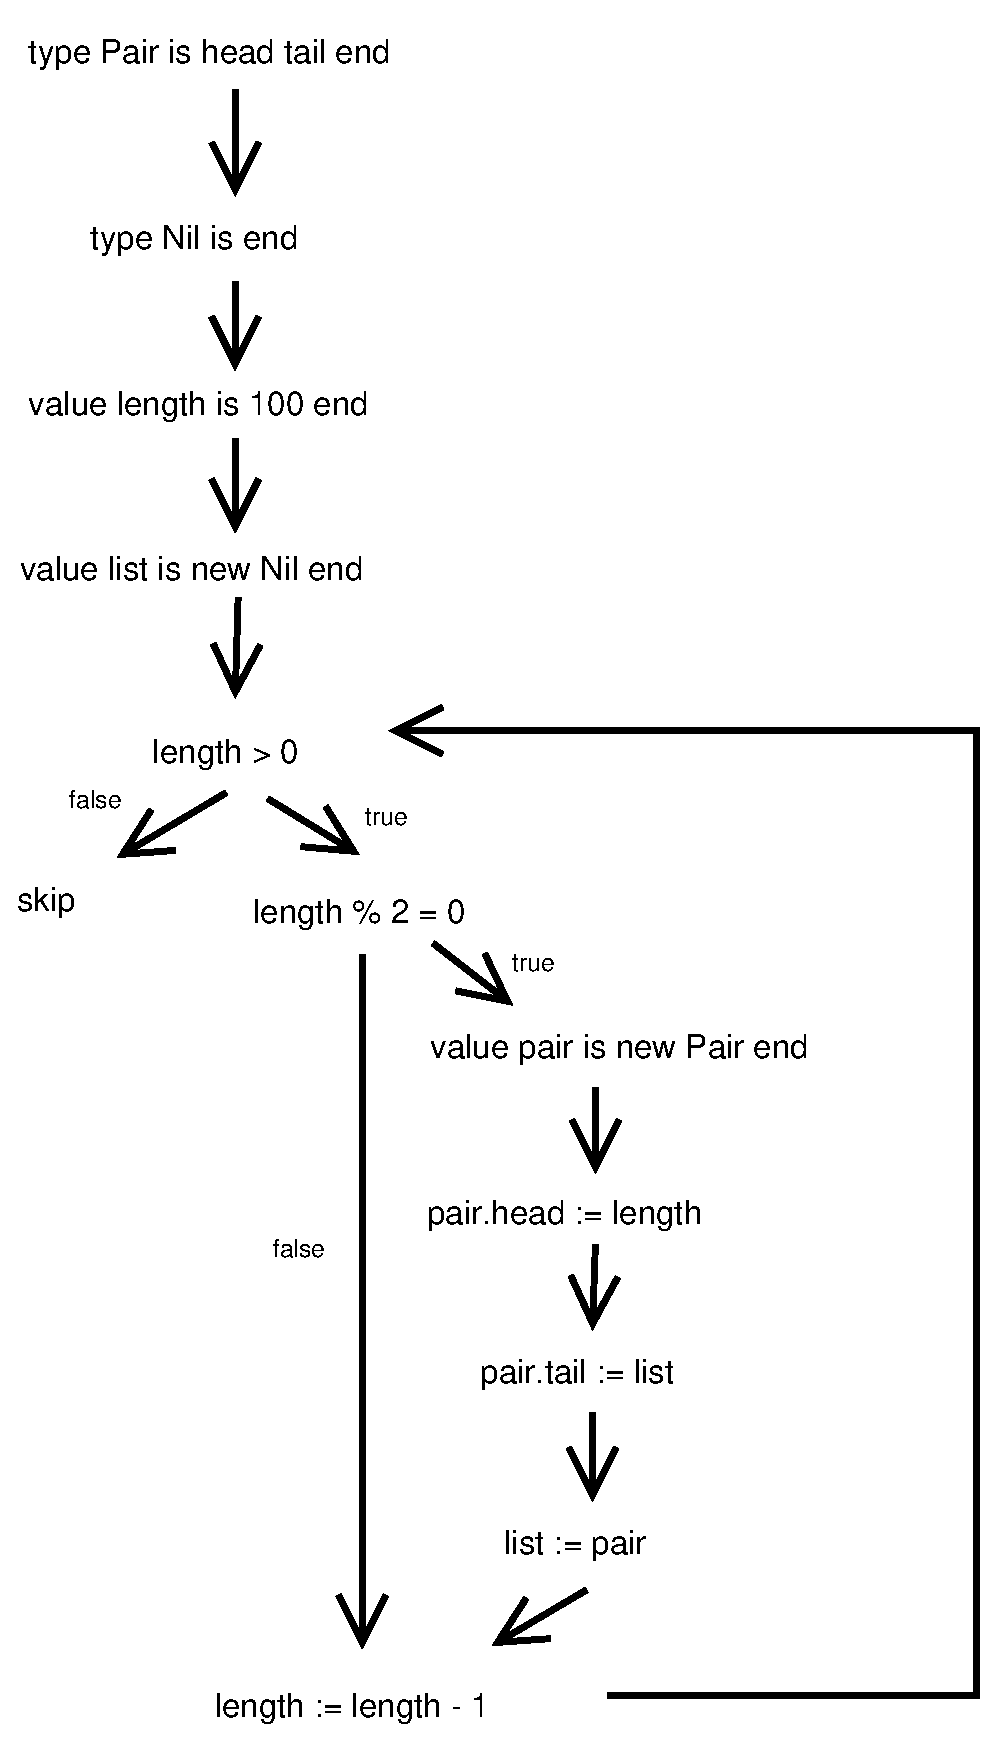
\psfig{file=Program.eps,height=10cm,width=7cm}
\end{center}
\caption{An example Flow graph}
\label{Program}
\end{figure}

Figure \ref{Program} shows an example flow graph corresponding to the
example XCom program given in section \ref{Intro}. Note that a {\tt while}
loop is represented as a test node whose {\it true} edge eventually
leads back to the test node.

XMF provides a packages called {\tt Graph} that provides a basic collection
of graph structures and operations. A graph node is created: {\tt Node(l)}
where {\tt l} is the label on the graph node. A graph edge is created:
{\tt Edge(l,s,t)} where {\tt l} is the label on the edge, {\tt s} is the
source node for the edge and {\tt t} is the target node for the edge. 

A graph is created: {\tt Graph(N,E)} where {\tt N} is a set of nodes and
{\tt E} is a set of edges. The graph shown in figure \ref{Program} is 
constructed as follows where classes {\tt Node} and {\tt Edge} have been 
specialized appropriately:
\begin{verbatim}
let n1 = Statement("type Pair is head tail end");
    n2 = Statement("type Nil is end");
    n3 = Statement("value length is 100 end");
    n4 = Statement("value list is new Nil end");
    n5 = Guard("length > 0");
    n6 = Guard("length % 2 = 0");
    n7 = Statement("value pair is new Pair end");
    n8 = Statement("pair.head := length;");
    n9 = Statement("pair.tail := list;");
    n10 = Statement("list := pair;");
    n11 = Statement("length := length - 1;");
    n12 = Statement("skip") then
    e1 = Next(n1,n2);
    e2 = Next(n2,n3);
    e3 = Next(n3,n4);
    e4 = Next(n4,n5);
    e5 = True(n5,n6);
    e6 = True(n6,n7);
    e7 = Next(n7,n8);
    e8 = Next(n8,n9);
    e9 = Next(n9,n10);
    e11 = Next(n10,n11);
    e12 = Next(n11,n5);
    e13 = False(n6,n11);
    e14 = False(n5,n12)
in Graph(Set{n1,n2,n3,n4,n5,n6,n7,n8,n9,n10,n11,n12},
     Set{e1,e2,e3,e4,e5,e6,e7,e8,e9,10,e11,e12,e13,e14})
end
\end{verbatim}
Graphs provide an operation {\tt reduce} that takes a node {\tt n} and a
sub-graph {\tt H} such that {\tt G.reduce(n,H)} produces a new graph that
is the result of removing {\tt H} from {\tt G}, adding {\tt n} to the
new graph and re-linking to {\tt n} any edges left dangling when {\tt H} 
is removed.

\subsection{Flow Graph Patterns}

Flow graphs can represent the control flow of a wide variety of different
languages and are used to analyse the structure of programs. The basic
elements of flow graphs are very low level - just nodes (representing
statements and expressions) and edges (representing flow between computational
states and the outcome of tests).

The low-level nature of flow-graphs gives rise to a weak correspondence
between a given graph and the program it represents. The correspondence
can be considerably strengthened by identifying sub-graphs with specific
language features. This is done by identifying patterns in flow-graphs;
wherever the pattern occurs, it can be replaced by a single node.

The choice of patterns depends on the collection of program features that
we intend to work with. For the purposes of XCom we will capture the
following patterns: {\tt P} is a pair of statements performed in sequence;
{\tt C} is an if statement and {\tt W} is a while-loop. 

The rest of this section shows how the pattern matching facilities of XMF 
can be used to detect these patterns. We define a flow-graph {\em aspect}
to XMF graphs by adding reduction operations to the class {\tt Graph}.

The simplest case is detecting and reducing a {\tt P} node. This occurs 
when two statements are linked via a {\em next} edge. The reduction is
shown in figure \ref{PReduction}.

\begin{figure}
\begin{center}
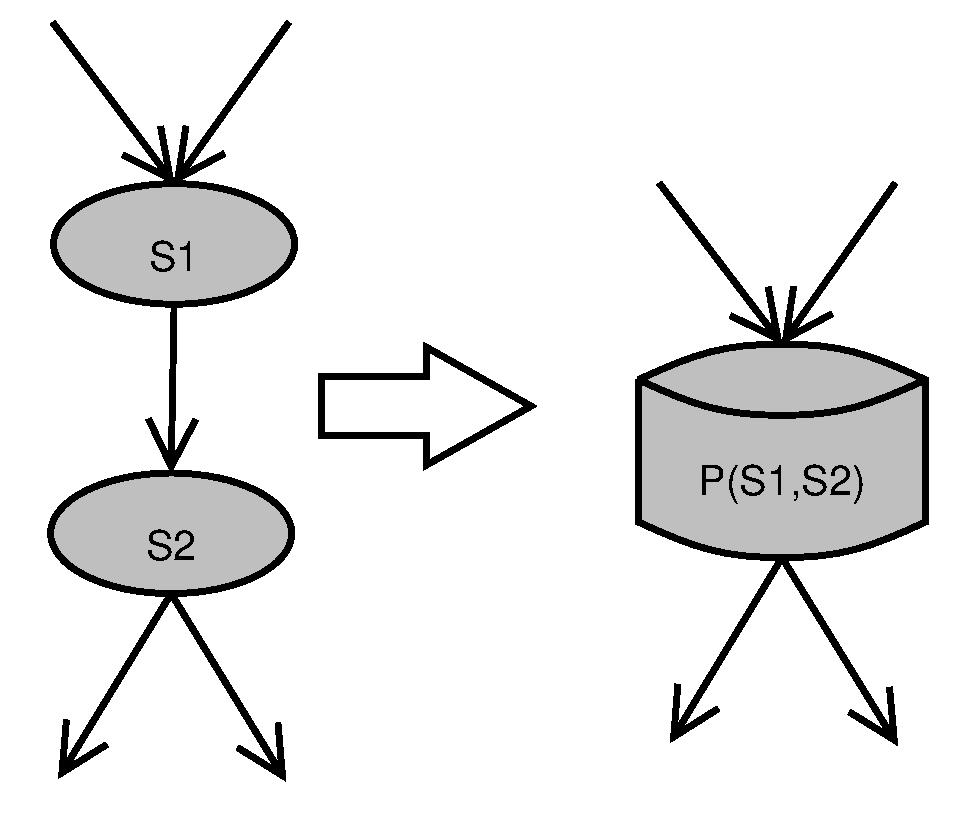
\includegraphics[scale=0.4]{P}
\end{center}
\caption{A P-Reduction Pattern}
\label{PReduction}
\end{figure}

\begin{verbatim}
context Graph
  @Operation reduceP():Graph
  
    @Case self of
    
      // Find two nodes with a then-edge
      // between them, replace with a P
      // node...
      
      Graph(N->including(n1 = Statement())
             ->including(n2 = Statement()),
            E->including(e = Next())
              when e.source() = n1 and
                   e.target() = n2)
      do
        self.reduce(P(e),Graph(Set{n1,n2},Set{e}))
      end
      
      // Otherwise, leave the receiver unchanged...
      else self
    end
  end
\end{verbatim}
A {\tt W} pattern corresponds to a {\tt while} loop and occurs when a test 
node has a true outcome that is a body statement
whose next leads back to the test. The false outcome leads to some root node
for the rest of execution. The reduction involves replacing the test and its body
with a {\tt W} node and adding a new next edge from the {\tt W} node to the root.
The reduction is shown in figure \ref{WReduction}.

\begin{figure}
\begin{center}
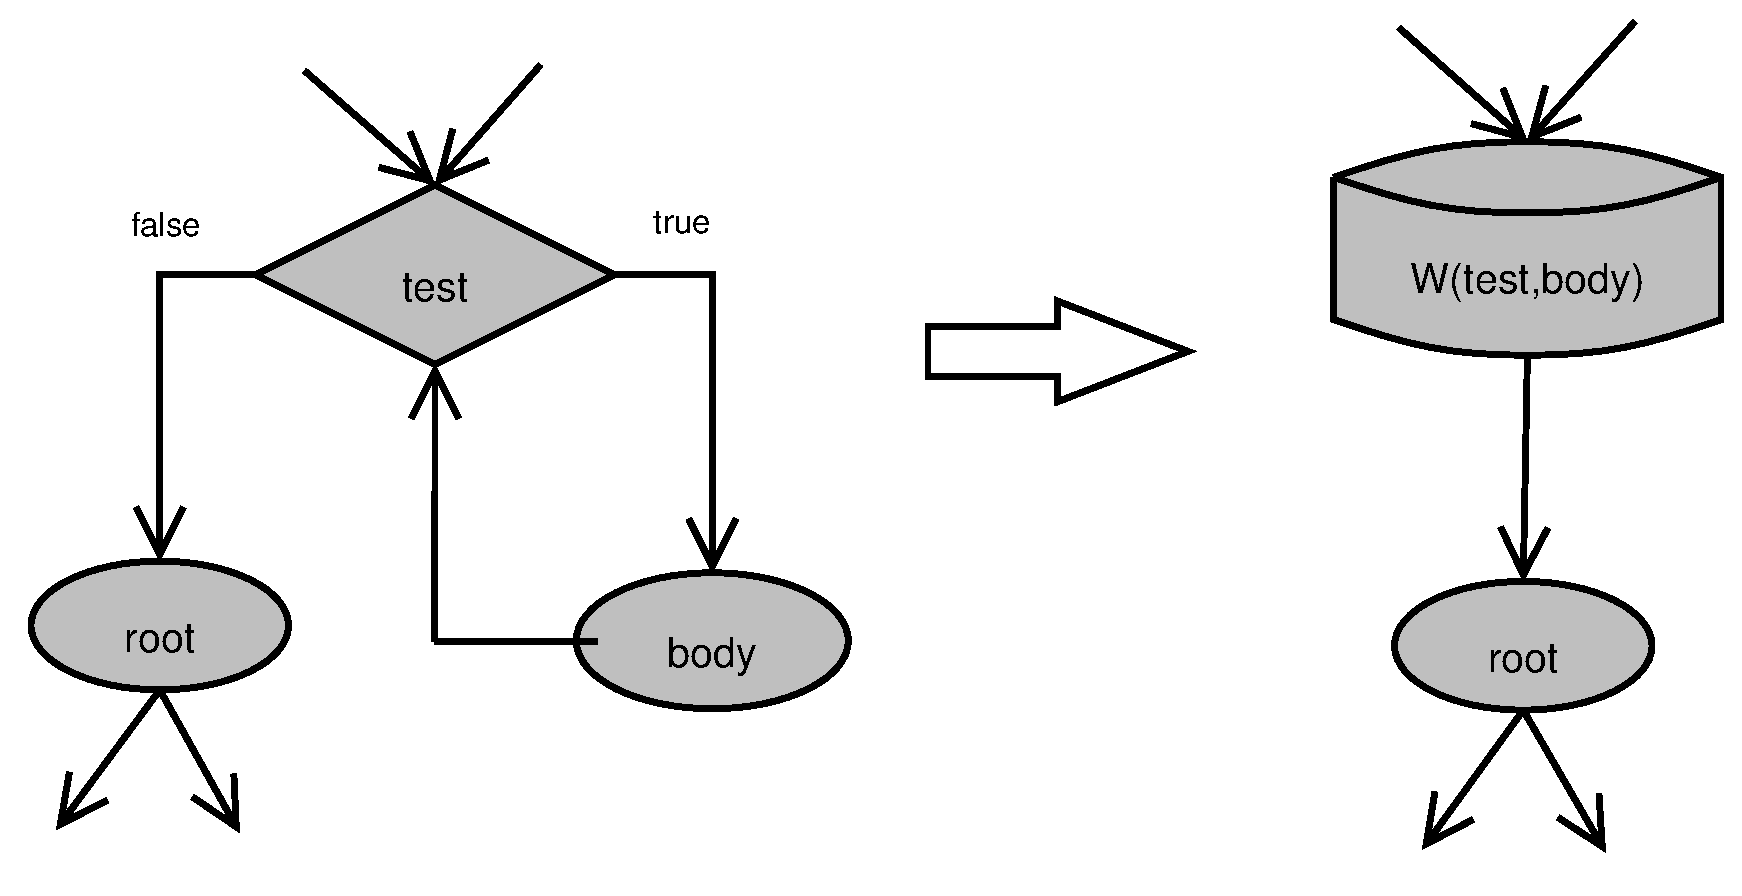
\includegraphics[scale=0.4]{W}
\end{center}
\caption{A W-Reduction Pattern}
\label{WReduction}
\end{figure}

\begin{verbatim}
context Graph
  @Operation reduceW():Graph
  
    @Case self of
    
      // Find a test node and a statement that are linked
      // via a true outcome and a loop back to the test.
      // Replace them with a W node ...
      
      Graph(N->including(test = Guard())
             ->including(body = Statement())
             ->including(root),
            E->including(enter = True())
             ->including(loop = Next())
             ->including(exit = False())
             when enter.source() = test and
                  enter.target() = body and
                  exit.source() = test and
                  exit.target() = root and
                  loop.source() = body and
                  loop.target() = test)
      do let Wnode = W(test,body);
             H = Graph(Set{test,body),Set{enter,loop,exit}) then
             newEdge = Next(Wnode,root)
         in self.reduce(Wnode,H).addEdge(newEdge)
         end
      end
      
      // Otherwise, leave the receiver unchanged...
      else self
    end
  end
\end{verbatim}
A {\tt C} pattern corresponds to an {\tt if} statement and occurs when there
is a test node leading to two nodes both of which lead to a single root node.
This forms a diamond pattern with the test node at one end. The test, then
and else parts of the graph are removed and replaced with a {\tt C} node.
The reduction is shown in figure \ref{CReduction}.

\begin{figure}
\begin{center}
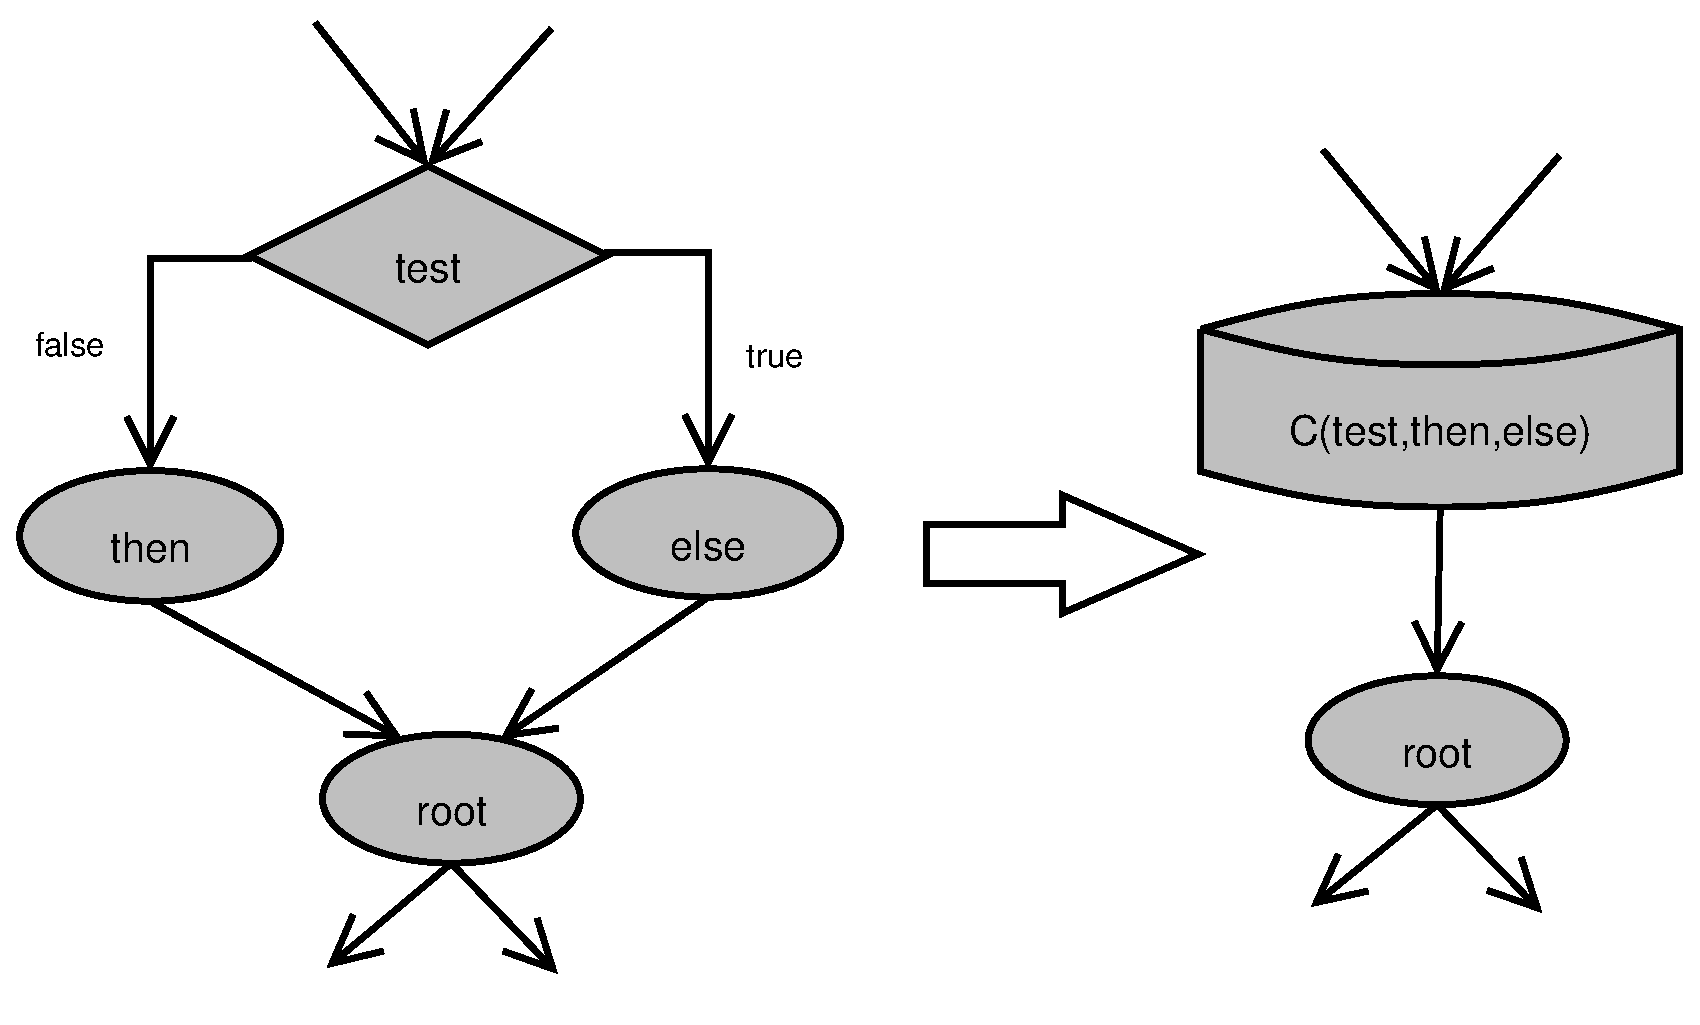
\includegraphics[scale=0.4]{C}
\end{center}
\caption{A C-Reduction Pattern}
\label{CReduction}
\end{figure}

\begin{verbatim}
context Graph
  @Operation reduceC():Graph
    @Case self of
      Graph(N->including(test = Guard())
             ->including(thenNode)
             ->including(elseNode)
             ->including(root),
            E->including(trueEdge = True())
             ->including(falseEdge = False())
             ->including(endThen = Next())
             ->including(endElse = Next())
                when trueEdge.source() = test and
                     trueEdge.target() = thenNode and
                     falseEdge.source() = test and
                     falseEdge.target() = elseNode and
                     endThen.source() = thenNode and
                     endThen.target() = root and
                     endElse.source() = elseNode and
                     endElse.target() = root)
      do
        let Cnode = C(trueEdge,falseEdge);
            H = Graph(Set{test,thenNode,elseNode},
                      Set(trueEdge,falseEdge,endThen,endElse}) then
            e = Next(Cnode,root)
        in self.reduce(Cnode,H).addEdge(e)
        end
      end
      
      else self
    end
  end
\end{verbatim}
Equality on graphs is defined in terms of the labels on the nodes and edges.
Two graphs {\tt G} and {\tt H} are equal when they have the same number of
nodes, when the respective sets of labels are equal, when the edges of {\tt G} 
correspond to the edges of {\tt H} in terms of the source and target nodes and 
when the respective sets of edge labels are equal. 

Graph reduction can involve more than one step. For example, certain configurations
of graph require a {\tt P} reduction to occur before a {\tt C} reduction can
occur. In order to reduce a graph fully we continually perform a reduction until
no further reductions can take place:
\begin{verbatim}
context Graph
  @Operation reduce():Graph
    let G = self.reduceP().reduceW().reduceC()
    in if G.equals(self)
       then G
       else G.reduce()
       end
    end
  end
\end{verbatim}
                
\subsection{Flow Graph Diagrams in XMF}

XMF provides a library of diagramming elements. A diagram consists of graph where nodes and edges
are labelled with display elements. Flow graphs consist of two types of node: statement nodes and
guard nodes; and, three types of edge: true edges, false edges and next edges. A diagram defines
a collection of tools that are used to create nodes and edges via the mouse. This section provides
an overview of how flow-graph diagrams are defined using the XMF diagramming package.

\begin{verbatim}
import Clients;
import Diagrams;

context Commands
  @Package Diagrams
    @Class Statement extends Node 
      @Attribute statement : Text end
    end
    @Class Guard extends Node 
      @Attribute test : Text end
      @Attribute line : Line end
    end
    @Class True extends Edge end
    @Class False extends Edge end
    @Class Next extends Edge end
    @Class FlowGraphDiagram extends Diagram end
  end
\end{verbatim}
A statement node contains a display element of type {\tt Text} that contains
the statement as a string. A diagram text element can be edited by selecting it 
with the mouse and typing. Each node has a position, a size and a right-click
menu, all of these are initialised when the node is created:
\begin{verbatim}
context Statement
  @Constructor(x,y)
     self.width := 150;
     self.height := 16 + 10;
     self.initRightClickMenu()
  end
\end{verbatim}
When a diagram {\tt Node} is added to a diagram, its {\tt addDisplays} operation 
is called to populate the node with display elements which are used to render the
node on the diagram. A {\tt Text} display has some text, an {\tt (x,y)} position
relative to its container and a boolean value determining whether or not it can be 
edited:
\begin{verbatim}
context Statement
  @Operation addDisplays()
    self.statement := Text("skip",5,5,true);
    self.add(dec)
  end
\end{verbatim} 
A diagram node contains a number of ports. A port is used to connect edges to the node
on the diagram. A port is not displayed on the diagram but has a position relative to
its containing node and a size. The operation {\tt addPorts} is called when a node
is added to a diagram:
\begin{verbatim}
context Statement
  @Operation addPorts()
    self.add(Port(0,0,width,height))
  end
\end{verbatim}
A node may be resized on a diagram by selecting it with the mouse and dragging an 
edge or a corner. When this occurs, the {\tt resize} operation of the node is
called. It is the responsibility of the node to resize any elements it contains;
the default behaviour defined by {\tt Node} is to update the {\tt width} and {tt height}
attributes:
\begin{verbatim}
context Statement
  @Operation resize(width,height)
    @For d in displays do
      d.resize(width,height)
    end;
    super(width,height)
  end
\end{verbatim}
A guard node is similar to a statement node except that the test is displayed with a 
line underneath:
\begin{verbatim}
context Guard
  @Operation addDisplays()
    self.line := Line(0,16 + 5,50,16 + 5);
    self.exp := Text("true",5,5,true);
    self.add(exp);
    self.add(line)
  end
\end{verbatim}
The {\tt resize} operation of a guard node must deal with the line:
\begin{verbatim}
context Guard
  @Operation resize(width,height)
    line.resize(width,0);
    @For port in ports do
      port.resize(width,height)
    end;
    super(width,height)
  end
\end{verbatim}
A true edge adds a non-editable label to the end of the edge. The constructor for an edge is
supplied with the source and target {\em ports} owned by the nodes at the respective
ends:
\begin{verbatim}
context True
  @Constructor(source,target) 
    self.init(Seq{source,target,0,Edge::arrow});
    self.add(Label("true","end",10,10,false))
  end
\end{verbatim}
A diagram manages a graph of nods and edges. In addition the diagram manages a collection
of tools that allow a user to interactively create instances of nodes and edges. The
tools are divided into two catageories: edge tool groups and node tool groups. The
operations {\tt defineEdgeToolGroups} and {\tt defineNodeToolGroups} are called automatically
when a diagram is created to set up the various creation tools.

Edge creation is defined by defining {\em new handlers} for each edge type. A handler is
an operation that will be supplied with the source and target ports when the user selects
the tool button and draws an edge between two nodes. Each handler then performs some 
actions that are specific to the edge type:
\begin{verbatim}
context FlowGraphDiagram
  @Operation defineEdgeToolGroups()
    let newFalse = 
          @Operation(sourcePort,targetPort) 
            self.newFalse(sourcePort,targetPort) 
          end;
        newNext = 
          @Operation(sourcePort,targetPort) 
            self.newNext(sourcePort,targetPort) 
          end;
        newTrue = 
          @Operation(sourcePort,targetPort) 
            self.newTrue(sourcePort,targetPort) 
          end
    in self.defineToolGroup("New Edge");
       self.defineNewHandler("New Edge","False",true,"False.gif",newFalse);
       self.defineNewHandler("New Edge","Next",true,"Next.gif",newNext);
       self.defineNewHandler("New Edge","True",true,"True.gif",newTrue)
    end 
  end
\end{verbatim}
When a new edge is created, it is added to the graph managed by the diagram using {\tt add}.
The {\tt new} operation of the edge causes the edge to appear on the diagram:
\begin{verbatim}
context FlowGraphDiagram
  @Operation newFalse(sourcePort,targetPort)
    let edge = False(sourcePort,targetPort)
    in edge.new(self);
       self.addEdge(edge);
       edge
    end
  end
\end{verbatim}
Node tool groups are defined in a similar way to edge tool groups. The node handlers are
supplied with the x and y co-ordinates of the mouse position when the node is created:
\begin{verbatim}
context FlowGraphDiagram   
  @Operation defineNodeToolGroups()
    let newStatement = 
          @Operation(x,y)
            self.newStatement(x,y)
          end;
        newGuard = 
          @Operation(x,y)
            self.newGuard(x,y)
          end
    in self.defineToolGroup("New Node");
       self.defineNewHandler("New Node","Statement",false,"Statement.gif",newBlock);
       self.defineNewHandler("New Node","Guard",false,"Guard.gif",newGuard)
    end
  end
\end{verbatim}
A node is created, added to the diagram and displayed in the same way as an edge:
\begin{verbatim}
context FlowGraphDiagram
  @Operation newStatement(x,y)
    let node = Statement(x,y)
    in self.add(node);
       node.new(self)
    end
  end
\end{verbatim}

\section{Graphical to Abstract Syntax Mapping}

\begin{verbatim}
@Operation transform(x)
  @Case x of
    Graph(N,E) do 
      Block(self.transform(N))
    end
    Statement(statement) do
      Seq{self.parseStatement(statement)}
    end
    P(e) do
      self.transform(e.sourceNode()) + 
      self.transform(e.targetNode())
    end
    C(trueEdge,falseEdge) do
      Seq{If(test,Block(thenPart),Block(elsePart))}
        where 
          test = self.parseExp(trueEdge.sourceNode().exp());
          thenPart = self.transform(trueEdge.targetNode()),
          elsePart = self.transform(falseEdge.targetNode())}
    end
    W(Guard(exp),body) do Seq{While(test,Block(statements))}
      where
        test = self.parseExp(exp);
        statements = self.transform(body)
    end
    N->including(n) do
      self.transform(n) + 
      self.transform(N)
    end
    Set{} do Seq{} end
  end
end
\end{verbatim}

\section{Conclusions}

This note has shown how XMF can be used to define the operational semantics of languages. We
have shown how to implement an interpreter for a simple language and how to translate the
language to existing XMF languages. We have discussed a number of different issues relating to
language translation, in particular how much work is performed statically and how much is left
to run-time.



\end{document}